\pdfoutput=1
\documentclass[11pt]{article}
% Renyi: the article (decision AW45 iii). Built with `latexmk -pdf renyi`
% in this directory; see README.md for the arXiv submission.
\usepackage[a4paper,margin=2.6cm]{geometry}
\usepackage[T1]{fontenc}
\usepackage[utf8]{inputenc}
\usepackage{lmodern}
\usepackage{microtype}
\usepackage{booktabs}
\usepackage{listings}
\usepackage{xcolor}
\usepackage{url}
\usepackage{tikz}
\usetikzlibrary{positioning,arrows.meta}
\usepackage[numbers,sort&compress]{natbib}
\usepackage[hidelinks]{hyperref}

\lstdefinelanguage{Renyi}{
  morekeywords={module,purpose,import,exposing,public,function,returns,or,fails,with,needs,for,any,where,can,example,is,let,be,mutable,change,to,if,then,else,end,otherwise,fail,return,each,in,sum,collect,count,group,by,sorted,descending,match,when,type,has,one,of,test,check,replays,at,most,per,run,minute,hour,day,only,crash,continue,ignore,and,not,nothing,true,false,expose,as,tool},
  sensitive=true,
  morecomment=[l]{\#},
  morestring=[b]",
}
\lstset{language=Renyi,basicstyle=\small\ttfamily,keywordstyle=\bfseries,
  commentstyle=\itshape\color{gray},stringstyle=\color{black},
  columns=fullflexible,keepspaces=true,breaklines=true,
  frame=none,xleftmargin=1em,aboveskip=0.6em,belowskip=0.6em,
  literate={->}{{$\rightarrow$}}2}

\title{Renyi: A Scripting Language for AI Agents\\
  with Declared, Enforced and Recorded Effects}
\author{Zhe Zhang\thanks{Renyi-lang, \url{https://renyi-lang.org}.
  Correspondence: \texttt{zhezhang.dev@gmail.com}.}
  \and Brandon Mocco\thanks{Renyi-lang.}}
\date{October 2026}

\begin{document}
\maketitle

\begin{abstract}
AI agents write small programs that glue services together, and the
person who runs one wants to know what it can touch before it runs and
what it did after. A script in a general-purpose language answers
neither. Renyi is a statically typed scripting language in which every
function signature declares its effects as capabilities with scopes and
budgets. The checker refuses a function that uses what it does not
declare, the grant of \texttt{main} is the whole program's authority,
dependencies included, and at run time every effect passes one boundary
in the virtual machine where the grant, the budgets and the provenance
guards are checked. The same boundary records a run as data, so that it
can be replayed offline, narrated through the program's own
\texttt{purpose} clauses and reproduced on another machine. The syntax
is a regular subset of English with one spelling per concept, named
arguments, no exceptions and a fix in every diagnostic, and its rules
were chosen by measuring language models reading and writing it. Three
statements hold of the rules and are mechanized in Lean 4. The declared
authority bounds every effect, a guarded value leaves only through its
sinks, and a replay of a recording makes the same calls with the same
answers. On AgentDojo's 629 injection cases, 90.8\% of the injected
goals need a capability, a scope or a count outside what the benign
task's program declares, so a program that passed review for the task
cannot carry them out. Every example workflow's recording reproduces on
another operating system, agents given the language's one-page skill
file wrote four of five workflows clean within two attempts, five of
five with the toolchain's MCP server connected, and Claude
Sonnet 5.5 reading the cheat sheet alone predicts the output of corpus
programs at 90\% and explains them at 100\%.
\end{abstract}

\section{Introduction}

Language models now write programs on behalf of a person, a few dozen
lines that read files, call an API and print or save a result. The
person skims the program, runs it and looks at the output. Before the
run they would like to know what the program can do, to which paths and
hosts, and how often. After the run they would like to know what it
did, and whether they can run it again and get the same answer.

A general-purpose scripting language gives neither answer cheaply. Any
line of a Python program may open any file or socket, an import may do
so at load time, and a dependency update may add a network call that
nothing in the program's text shows. Sandboxes answer the first
question from outside the program, per process (Deno's permission
flags~\citep{deno}, containers, WebAssembly runtimes), and the second
not at all. Effect systems answer the first question in the
type~\citep{leijen2014koka,brachthauser2020effekt} but say nothing
about a run. The recent languages for agents' programs
(Section~\ref{sec:related}) separate the logic from the calls, for
approval or for speed, and leave both questions open at the signature.

Renyi gives both answers (Figure~\ref{fig:overview}). A function's
signature lists what it needs, the checker refuses a body that uses
more, directly or through a call, and the signature of \texttt{main} is
the grant of the whole program, dependencies included. Every effect of
a run passes one boundary in the VM, and the boundary's record is what
answers the second question. The syntax fits on one page of under 3,000
tokens, and its rules were settled by measuring language models reading
and writing it. Section~\ref{sec:design} gives the design,
Section~\ref{sec:implementation} the implementation and
Section~\ref{sec:evaluation} the measures, among them the authority gap
of a benchmark of injection attacks, the share of its attacks that need
more authority than the benign task's program declares.

\begin{figure}[tbp]
\centering
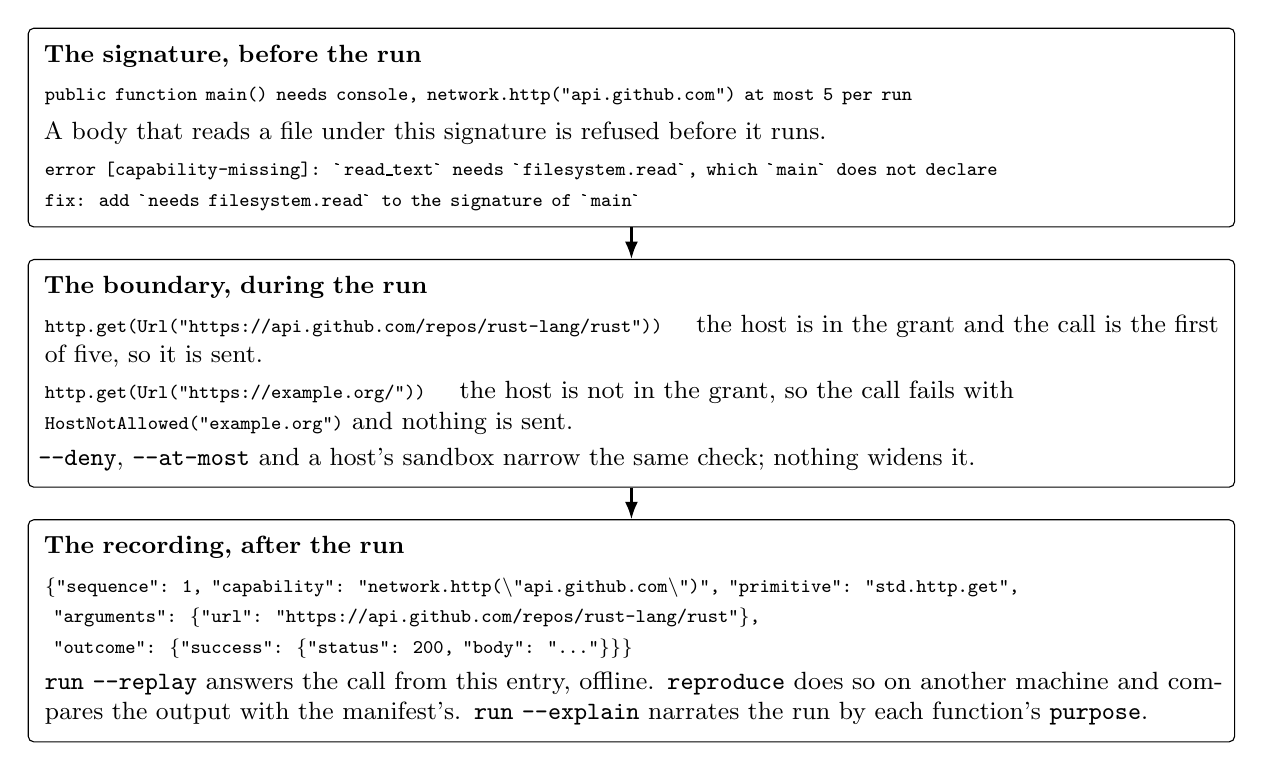
\begin{tikzpicture}[
  font=\small,
  box/.style={draw,rounded corners=2pt,align=left,inner sep=6pt,text width=14.9cm},
  arrow/.style={-{Latex[length=2.2mm]},thick},
]
\node[box] (sig) at (0,0) {%
  \textbf{The signature, before the run}\\[3pt]
  {\scriptsize\texttt{public function main() needs console, network.http("api.github.com") at most 5 per run}}\\[3pt]
  A body that reads a file under this signature is refused before it runs.\\[2pt]
  {\scriptsize\texttt{error [capability-missing]: \textasciigrave read\_text\textasciigrave{} needs \textasciigrave filesystem.read\textasciigrave, which \textasciigrave main\textasciigrave{} does not declare}}\\
  {\scriptsize\texttt{fix: add \textasciigrave needs filesystem.read\textasciigrave{} to the signature of \textasciigrave main\textasciigrave}}};
\node[box,below=0.4cm of sig] (vm) {%
  \textbf{The boundary, during the run}\\[3pt]
  {\scriptsize\texttt{http.get(Url("https://api.github.com/repos/rust-lang/rust"))}}
  \quad the host is in the grant and the call is the first of five, so it is sent.\\[2pt]
  {\scriptsize\texttt{http.get(Url("https://example.org/"))}}
  \quad the host is not in the grant, so the call fails with
  {\scriptsize\texttt{HostNotAllowed("example.org")}} and nothing is sent.\\[2pt]
  \texttt{-{}-deny}, \texttt{-{}-at-most} and a host's sandbox narrow the
  same check; nothing widens it.};
\node[box,below=0.4cm of vm] (rec) {%
  \textbf{The recording, after the run}\\[3pt]
  {\scriptsize\texttt{\{"sequence": 1, "capability": "network.http(\textbackslash"api.github.com\textbackslash")", "primitive": "std.http.get",}}\\
  {\scriptsize\texttt{\ "arguments": \{"url": "https://api.github.com/repos/rust-lang/rust"\},}}\\
  {\scriptsize\texttt{\ "outcome": \{"success": \{"status": 200, "body": "..."\}\}\}}}\\[2pt]
  \texttt{run -{}-replay} answers the call from this entry, offline.
  \texttt{reproduce} does so on another machine and compares the output
  with the manifest's. \texttt{run -{}-explain} narrates the run by each
  function's \texttt{purpose}.};
\draw[arrow] (sig) -- (vm);
\draw[arrow] (vm) -- (rec);
\end{tikzpicture}
\caption{One program at the three places Renyi acts: the starter
workflow of Figure~\ref{fig:program}, with the toolchain's own texts.
The checker refuses a body that uses what the signature of
\texttt{main} does not declare; the boundary in the VM admits or
refuses each primitive call against the grant; the boundary's record
is what a replay, a reproduction and a narration read.}
\label{fig:overview}
\end{figure}

\section{The design}
\label{sec:design}

Four decisions, taken before any tool was written, carry the rest. A
function without a \texttt{needs} clause is pure, and time and
randomness are capabilities, so the runtime sees every effect at one
boundary. Every value is immutable and every binding owns its value. A
function captures nothing, a top-level binding is a constant, and a
value reaches another only by copy or move, so the value graph is
acyclic and a service's state lives outside the program. A definition's
identity is the hash of its canonical form, so a rename changes nothing
and a changed body changes everything that depends on it. And every
module and every public definition carries a \texttt{purpose} line, so
a run can be narrated in its author's words.

\subsection{A program}

Figure~\ref{fig:program} shows a workflow from the toolchain's starter
pack, shortened. The reviewer reads the \texttt{needs} of \texttt{main}
first. The program prints to the console, reads its arguments and makes
at most five HTTP requests per run to one host, and nothing else can
happen, whatever the rest of the file says.

\begin{figure}[tbp]
\begin{lstlisting}[basicstyle=\footnotesize\ttfamily]
module api_digest
  purpose: Fetch a repository's public numbers from the GitHub API and print a one-line digest.

import std.console
import std.environment
import std.http exposing Url, HttpError
import std.json exposing JsonError

public type DigestError is one of
  purpose: Why the digest could not be printed.
  Unreachable(detail: Text)
  BadResponse(detail: Text)
end

public function fetch_repository(name: Text)
  returns Repository
  or fails with HttpError or JsonError
  needs network.http("api.github.com")
  purpose: Download the record of the repository "owner/name".

  let response be http.get(Url("https://api.github.com/repos/{name}")) otherwise fail
  let repository: Repository be json.parse(response.body) otherwise fail
  return repository
end

public function main()
  or fails with DigestError
  needs console, environment, network.http("api.github.com") at most 5 per run
  purpose: Print the digest of the repository named by the argument, rust-lang/rust by default.

  let arguments be environment.arguments()
  let name be arguments.at(0) otherwise "rust-lang/rust"
  let repository be
    match fetch_repository(name)
      when success(found) then found
      when failure(error: HttpError) then fail with Unreachable(detail: error.to_text())
      when failure(error: JsonError) then fail with BadResponse(detail: error.to_text())
    end
  ...
end
\end{lstlisting}
\caption{A starter workflow, its record type and the end of the body left
out. The signature of \texttt{main} is the program's grant. The function
it calls declares the host it needs, and the grant covers it.}
\label{fig:program}
\end{figure}

\subsection{Capabilities in signatures}
\label{sec:capabilities}

\begin{sloppypar}
A \texttt{needs} clause lists capabilities. The kinds are
\texttt{console}, \texttt{environment}, \texttt{time}, \texttt{random},
\texttt{filesystem.read}, \texttt{filesystem.write},
\texttt{network.http}, \texttt{network.socket}, \texttt{process},
\texttt{screen}, \texttt{foreign} and \texttt{python}, the modules of
the standard library that have effects. A capability may
carry a scope (a path, a host, or a parameter of the function, so that
a library function can say \texttt{needs network.http(host)}), a budget
(\texttt{at most $n$ per} second, minute, hour, day or run, or
\texttt{at most $n$ of} a parameter \texttt{per} unit, which sums that
argument instead of counting calls) and a guard (\texttt{only to} a
sink).
\end{sloppypar}

Capabilities form a tree, in which \texttt{filesystem} covers
\texttt{filesystem.read}, and scopes an order, in which a path prefix
contains its sub-paths, a host contains only itself and a capability
without a scope contains every scope. A granted capability covers a
needed one when its path is the same or an ancestor and its scope
contains the needed scope. The checker's rule is coverage. A body may
use, directly or through a call, only what its signature covers, a
test's head covers its body the same way, and the grant of
\texttt{main} must cover every function the program reaches, in its own
files and in its packages. The diagnostic names the callee, the
capability and the fix (Figure~\ref{fig:overview}). Across a package
boundary only the kind is checked, since a library cannot know its
caller's hosts; the scope is checked at the call.

At run time the effective grant of a function is the program's grant
intersected with the scopes declared along the call chain, and every
primitive compares the actual host or path with it when called. A
general HTTP client package that declares \texttt{network.http} without
a scope therefore serves a program that grants one host. The command
line narrows the same way, with \texttt{-{}-deny},
\texttt{-{}-allow-host} and \texttt{-{}-at-most}, and so does the
embedding API, in which a host loads a module under a grant narrower
than the module's own \texttt{main} declares, with a memory budget kept
by a counting allocator. Nothing from outside can widen a grant. A
budget is a counter per capability and scope, a sliding window for a
unit of time and a plain count for the run.

A guard is a taint of constant cost. The guards of a run are the
capabilities of the grant that carry \texttt{only to}, at most 64, and
each is one bit of the one-word origin every value carries. A primitive
call under a guarded capability tags its result with the guards that
cover it and with its arguments' origins, and every operation of the VM
tags its result with the union of its operands'. Before an outgoing
call the boundary requires every guard in the arguments' origins to
name a sink covering the call, and otherwise fails the call with
\texttt{Guarded(origin, sink)} before anything leaves. A recording
stores plain values and spells the guards in its header, so a replay
derives the same origins. Guards track explicit flow only; a branch on
a guarded value does not tag what the branch computes.

\subsection{Packages}

A package's effect manifest is computed from its sources by
\texttt{renyi index}, which derives every public function's transitive
effects and failure types, and the client recomputes it on every fetch
and refuses a package whose claimed manifest differs. \texttt{renyi add}
prints the effects a dependency brings before anything is written.
\texttt{renyi update} diffs the manifests of the old and the new version
and refuses one whose effects widen unless \texttt{-{}-accept-effects}
is given and \texttt{main} covers the new capability. The lockfile pins
content hashes, so a republished version with new effects is a different
hash and a refused update, and \texttt{renyi audit} lists every locked
dependency's effects against the program's grant. A package that calls
native code needs \texttt{foreign}, and a program that grants it is told
so the first time it runs.

\subsection{Recording, replay, narration, reproduction}
\label{sec:recording}

A run is a function of its code, its dependencies and the answers its
primitive calls received, because everything else is pure. There is no
ambient I/O, no reflection and no foreign call without a capability;
time and randomness are answered at the boundary like any other call;
maps and sets iterate in insertion order; decimal and float arithmetic
follow their standards; tasks run one after the other, in the order of
the text. A recording is therefore an oracle for the run.

\texttt{renyi record} writes a run as a JSON document, one entry per
primitive call with its arguments and its outcome
(Figure~\ref{fig:overview}). \texttt{renyi run -{}-replay} answers every
call from it and touches nothing outside the process. A call is matched
by primitive and arguments, and by sequence only when several entries
match; the recording's grant must be covered by the grant it is
replayed under, so a recording cannot bring an effect past a test's
\texttt{needs}. Arguments and outcomes are written by the library's JSON
rules, so a person or an agent can read and edit a recording, and a
replay decodes it against the declared types, so a response whose shape
no longer fits fails as it would in production. A recording can be
redacted by name and keeps a placeholder with the hash of what was
removed.

The recording's header is a manifest. It names the toolchain, the
content hash of \texttt{main}'s closure, every dependency's version and
hash, the grant, the arguments, the outcome and the hash of the output.
\texttt{renyi reproduce} refuses a program whose \texttt{main} does not
hash as the manifest says, warns when the toolchain differs, refuses
when the dependencies differ, replays, and compares the outcome and the
output, naming the first call that differed. A \texttt{replays} test
pins a function with effects to a recording the same way, and
\texttt{-{}-refresh} records it live once.

\subsection{Three statements}
\label{sec:statements}

These rules keep the properties below. Each is proved on paper over an
abstract machine whose steps are pure steps and primitive calls
(\texttt{docs/research/}\allowbreak\texttt{core-calculus.md} in the
repository), and mechanized in Lean 4 (\texttt{formal/}, Lean core
alone, built by the continuous integration with no \texttt{sorry}, a
model per theorem).

\textbf{Theorem 1 (authority bound).} In every run of a program the
checker accepts, every effect is covered by the run's grant, the
\texttt{needs} of \texttt{main} narrowed by the host, and its kind by
the \texttt{needs} of \texttt{main}. Within one checked program a
primitive is refused on its scope alone, its kind being covered along
the whole chain.

\textbf{Theorem 2 (guards admit only their sinks).} A value's origins
are exactly its explicit provenance, the guards whose data it was
computed from, and every primitive call that happens has, for every
guard in its arguments' provenance, a sink covering its effect.

\textbf{Theorem 3 (replay).} The replay of a recording makes the same
primitive calls with the same answers and produces the same output,
since every pure step is a function of the state and the recording
answers every call as the world did.

Each proof rests on the assumptions of Section~\ref{sec:recording} and
on the budgets and guards being decided by the state. Each assumption
is a sentence of the language reference, and a change to one is a
change to the statement. The Lean model of the third theorem starts the
replay from the live run's initial state, the one place the model asks
more than the statement.

\subsection{The surface}

The grammar is a W3C EBNF, frozen by decision and held equal to the
parser by a test that interprets it over the corpus. Each concept has
one spelling. \texttt{let $x$ be $e$} binds, \texttt{change $x$ to $e$}
is the only mutation, \texttt{is} and \texttt{is not} are the only
equality, every block ends with \texttt{end}, and the formatter has one
canonical layout. Values and functions are in lower snake case, and the
reserved words include the query vocabulary (\texttt{for each item in
items where \ldots\ sorted by \ldots\ collect}, \texttt{sum},
\texttt{count}, \texttt{group by}), so that a loop reads as a sentence.
One argument is positional and two or more are all named, in
declaration order; a function passed as a value is passed by name. A
function that can fail says \texttt{or fails with $E$}, and a call that
can fail or answer \texttt{nothing} takes \texttt{otherwise} on the same
line (\texttt{otherwise fail}, \texttt{otherwise $d$}, \texttt{otherwise
return}, \texttt{otherwise crash with "reason"}); there are no
exceptions. A binding must be read and a result used or
\texttt{ignore}d. A module and a public definition carry a
\texttt{purpose} line, and \texttt{example} lines on pure functions are
tests. Each rule is a diagnostic with a code and a fix, and the lexer,
the parser and the checker take the fix as an argument of every
diagnostic they raise, so none can be added without one.

\subsection{Where the guarantees stop}
\label{sec:limits}

Guards stop the wholesale exfiltration a prompt injection aims at, not
a covert channel. Implicit flow, timing and the size of what is sent are
not tracked, so a program can leak one bit per run through a branch,
and the budget on the sink bounds the rate. A path scope contains a
path by its text, with nothing resolved on disk, so a symbolic link
under a scope reaches wherever it points. What a \texttt{foreign} or a
\texttt{python} function does, once granted, is outside the VM's
guarantees, which is why both are capabilities a reviewer reads in the
grant. The sandbox isolates effects, time and memory but does not hide
timing or scheduling from the module. A recording holds what the
primitives answered, not what the world would answer today, so
\texttt{reproduce} shows that the program still computes the same output
from the same answers, not that the answers are still true.

\section{The implementation}
\label{sec:implementation}

\subsection{The toolchain and the VM}

The toolchain is one binary, \texttt{renyi}, written in Rust (103,194
lines at release 0.4.0), with a checker, a package client, a project
map, a workspace that a language server and a server for the Model
Context Protocol~\citep{mcp} keep between calls, the VM, a sandbox API,
a WebAssembly build and a C API with a Python binding. The standard
library is 16 modules declared in Renyi with native implementations in
the VM. The reference has one section per construct with the grammar
excerpt, the static rules with their codes and the run-time behaviour,
and a conformance suite of 67 cases runs against any \texttt{renyi}
binary on Linux and Windows for every push.

The checked tree is lowered to a stack bytecode, every operation
annotated with the type the checker inferred. The VM runs it on three
tiers. The interpreter runs every program first. A template tier
assembles, at a code object's first call, a fixed machine-code sequence
per operation over the interpreter's helpers and counts what it runs. A
code object that has run a fixed factor times its size is translated to
Cranelift IR~\citep{cranelift} on a background thread, or at a loop
header with on-stack replacement, after an abstract interpretation has
settled which operands and locals stay unboxed in registers, which
calls borrow their arguments where they lie and which push no frame
record. A hand-back rebuilds the interpreter's state wherever the
generated code cannot continue.

Every effect passes one function, \texttt{call\_native}, which checks
the effective grant and the budgets, records or replays the call, and
narrates it. The machine-code tiers call the library's pure primitives
(text, list, map and number operations) through in-place entries that
bypass it. \texttt{renyi build} writes an image, the bytecode with the
machine code of every function, which is mapped executable from the
file, and \texttt{build -{}-exe} appends the image to the binary as a
self-contained executable. The front end, the checker and the
interpreter also build for \texttt{wasm32}, which is how the project's
site runs the playground and a Doom-style game written in Renyi in the
browser.

\subsection{Memory}
\label{sec:memory}

The value graph is acyclic, since a value is immutable and reaches
another only by copy or move, so the VM counts references and needs no
tracing collector. A value is freed when its count reaches zero, so a
file or a connection closes as soon as it is dropped. A value whose
count is one is updated in place, so \texttt{change items to
items.append(item)} is a constant-time append when nothing else holds
the list, and the compiler marks the last read of every local as a
move, so an argument is handed over rather than copied. This is the
model of Perceus~\citep{reinking2021perceus}, with the acyclicity given
by the language. The language and its diagnostics speak of values
only; ownership stays inside the VM.

\subsection{The compiler written in Renyi}

The lexer, the parser, the checker and the bytecode emitter are
written again in Renyi (25,974 lines) and run by the Rust VM. Three
judges in the test suite hold them equal to the Rust toolchain on every
commit. The Renyi parser must print, byte for byte, what \texttt{renyi
parse -{}-json} prints on every program of the corpus, the conformance
suite, the compiler and the library, the Renyi checker what
\texttt{renyi check -{}-json} prints, with its exit status, on the
rejected programs too, and the Renyi compiler the bytecode file
\texttt{renyi compile} writes, that file of itself among them. The
compiler is also the toolchain's speed measure. The gate for switching
the binary's front end to it was three times the Rust front end's
instructions on checking the compiler's largest module, the VM's rounds
and two rounds of cuts in the compiler's sources brought the ratio to
2.96, and the Rust front end stays in the binary with the Renyi one as
its judged twin.

\subsection{Tooling}
\label{sec:identity}

Every definition is content-addressed, after Unison~\citep{unison}. Its
identity is the SHA-256 of its canonical text with its own name
replaced by a placeholder, every reference to another definition of the
project replaced by that definition's hash, and the library definitions
it uses appended with the library's version. A rename changes no hash,
and a changed body changes the hash of everything that depends on it.
The same hash is the code hash of the run manifest and the identity of
every record of the project map.

\texttt{renyi index} builds the map from the checked program, with the
signature, the effects, the failure types, the callers and callees, the
metrics and the hash of every module and definition. \texttt{index
-{}-diff} compares two maps, or a map and a revision, and lists the
changes with what each reaches and the version bump it forces.
\texttt{index -{}-chunks} writes the map as JSON Lines, one chunk per
definition with the hash of its text as its id, so that a host's
retrieval index changes exactly when a definition does. \texttt{renyi
mcp} serves the map, the checker, the formatter, the tests, the chunks
and the cheat sheet to an agent host, keeping the checked world of the
directory between calls, and \texttt{renyi lsp} serves editors from the
same world.

\texttt{renyi serve -{}-watch} runs a service and, when a file of its
project changes, checks the whole program again and runs \texttt{main}
again on the new version between two requests, with the listening
socket handed over. There is nothing to migrate, because a module has
no mutable state and no mutable value escapes a function; the state of
a service lives in its database, its files and its requests. The
reload's message is the semantic diff, and a version with errors leaves
the last good one serving. This is Erlang's hot code
loading~\citep{armstrong2003} without a replacement on a running stack,
and with the whole program checked before it serves.

\section{Evaluation}
\label{sec:evaluation}

The reproduction and the benchmarks were measured on release 0.4.0 on
2026-10-15. The first-run measure was taken on release 0.2.0 on
2026-10-14 with the skill file and the cheat sheet of that release,
and again on release 0.4.0 on 2026-10-17 with the MCP server
connected.

\subsection{Reproduction}

The starter pack's five workflows (a repository digest from Git, an API
digest from GitHub, an expense report from CSV files, a log triage, a
link check) were recorded on Windows 11 with the release binary
installed through \texttt{cargo install}, and reproduced under Linux
with the binary the project's \texttt{install.sh} put in place. All five
reproduced, with the recorded outcome and output.

\subsection{The authority gap}
\label{sec:gap}

Theorem 1 says what a program cannot do. The question for an agent's
program is how much of what an attacker wants falls outside it. A
prompt injection reaches the program through the data a tool returns
and asks for something the user did not, and in Renyi the program's
authority was declared and reviewed before the run, so the injected
goal is carried out only if it fits inside that authority. We call the
share of a benchmark's attacks that do not fit the smallest grant the
benign task's program can declare the \emph{authority gap}. It is a
property of the task and the attack, not of a model. For every pair in
the gap, no program that passed review for the task can carry out the
attack, whatever the model does once it runs, so the gap is the ceiling
of every defense that fixes authority before the run and says what is
left for the mechanisms that act during it.

We measured it on AgentDojo~\citep{debenedetti2024agentdojo}, the
benchmark of injection attacks on tool-using agents on which
Quasar~\citep{mell2025quasar} and CaMeL~\citep{debenedetti2025camel}
are evaluated, in its \texttt{v1} suites (banking, slack, travel,
workspace): 97 user tasks, 27 injection tasks, every user task of a
suite paired with every injection task of it, 629 pairs. Each task
declares a ground truth, the tool calls with their arguments that carry
it out, and the measure reads the task files as syntax trees and runs
nothing. A tool is a capability kind, and the argument naming a
recipient, a URL, a channel, a hotel, a file or a participant list is
its scope. The user task's grant is what its program can write in the
\texttt{needs} of \texttt{main}. It has every kind its ground truth
calls, a scope for a kind when every call's scope is a literal the
user's prompt spells out (a recipient read from a file is not
declarable), \texttt{at most $n$ per run} with $n$ the ground truth's
count, and \texttt{at most $A$ of amount per run} on a kind whose
amount is a literal the prompt spells out in every call, with $A$ their
sum. A pair
is blocked when the injection's calls need a kind the grant lacks, a
scope outside a declared one, more calls than the count or amounts
summing past the budget. Table~\ref{tab:gap} gives the result under
five grants, from the kinds alone to the ceiling of every literal as a
scope.

\begin{table}[t]
\centering
\begin{tabular}{lrrrrrr}
\toprule
Suite & pairs & kinds & + scopes & + counts & + amounts & ceiling \\
\midrule
banking & 144 & 72.9\% & 89.6\% & 91.0\% & 91.7\% & 98.6\% \\
slack & 105 & 81.9\% & 89.5\% & 89.5\% & 89.5\% & 97.1\% \\
travel & 140 & 81.4\% & 82.9\% & 82.9\% & 82.9\% & 82.9\% \\
workspace & 240 & 92.5\% & 96.7\% & 96.7\% & 96.7\% & 100.0\% \\
\midrule
all & 629 & 83.8\% & 90.8\% & 91.1\% & 91.3\% & 95.4\% \\
\bottomrule
\end{tabular}
\caption{The authority gap on AgentDojo \texttt{v1}, the share of (user
task, injection task) pairs whose attack does not fit the user task's
grant, under the kinds alone, with the scopes the prompt spells out,
with per-run counts, with budgets on the amounts the prompt spells out,
and with every literal as a scope, an upper bound that the amounts do
not move. Travel's 20 unblocked pairs under every grant are one
injection that only wants the agent to say something.}
\label{tab:gap}
\end{table}

The 35 pairs that fit the fourth grant are of two kinds. In 11 of them
the task's own sink is the attack's. A banking task names the
attacker's account as the user's new landlord, one asks for a password
change and the attack asks for another, and four slack tasks message
Alice and the attack sends Alice a link. In 24 the task itself reads
its sink from
the attacker's data, a bill's recipient, a page's address found in a
channel, people found by name, a file found by listing, or a calendar
event, which has no scope. No authority fixed before the run can
separate those. The recording and the narration after the run act on
them, and so does the reviewer who sees \texttt{send\_money} without a
scope and knows the bill chooses the recipient. The budget on an amount
is for the attacks that move as much money as possible; Renyi's budgets
counted calls when the measure was first made, the amount budget was
added since, and it blocks one pair, the only task whose prompt spells
its amount. The attacks that remain under any limit send 0.01 with the
user's data in the subject. The measure assumes a program fixed before
any effect, takes the ground truth as the task's authority, with the
kinds row as the floor and the ceiling row as the bound a broader review
could reach, and runs no model, so it says nothing about utility, which
CaMeL reports with a model in the loop. The data, the scripts and the
pinned output are in the repository, held by its continuous integration.

A model in the loop gives the same number. Claude Sonnet 5.5, given the
toolchain's skill sheet and cheat sheet, wrote a Renyi program for each
of the 97 user tasks against the suite's tools bound as Python modules,
one capability kind each, with at most three attempts and \texttt{renyi
check}'s diagnostics fed back. 96 tasks got a program the checker
accepts (55 at the first attempt, 38 at the second, 3 at the third). 75
of them call exactly the ground truth's tools, 13 call one it does not,
and 14 miss one it calls, among them the tasks whose steps are in the
email or the web page the program reads. Under the grants those
programs declare, 522 of their 622 pairs are blocked (83.9\%), against
518 (83.3\%) under the ground truth's kinds on the same pairs. The
declared grant is the call set, and the floor holds with a model in the
loop.

Run against the benchmark's own environments through the Python bridge
and judged by each task's own check, 54 of the 96 programs do their
task (56\%; 48 of the 75 whose call set is the ground truth's, 6 of the
21 others), each written once from the prompt and the declarations
without a look at the data. With the loop the toolchain is built for,
in which the program runs under \texttt{renyi record}, the model reads
the run and the recording and writes the program again, each version
is checked before it runs, and there are at most two turns, 81 of the
96 do their task (84\%), 27 repaired and none broken. The grant changed
in 9 programs and widened in 5, four of them by a tool the ground truth
calls, and 520 of the 622 pairs are blocked under the final grants
(83.6\%) against 522 under the first. The look at the data that repairs
the program does not loosen the grant. The sample, the programs, their
runs and the pinned reports are in the repository.

\subsection{First-run rate}

Five tasks of the workflows' kind (Table~\ref{tab:firstrun}) were each
given to a fresh agent, a Claude Code subagent allowed to read only the
starter pack's skill file and the one-page cheat sheet, with no MCP
server and no other file of the repository, and to run the release
binary. An attempt is one version of the program followed by
\texttt{renyi check}. Three tasks checked clean on the first attempt,
one on the second and one on the third, and the tests and the run
passed on the same attempt in every case, with the outputs checked by
each agent against an independent computation. Every failed attempt but
one was answered by a diagnostic whose fix the agent applied:
\texttt{unknown-field} on \texttt{path.name} proposed \texttt{.name()},
and \texttt{error-not-declared} named the error type \texttt{JsonError}
that \texttt{main} had to declare. The exception was the second attempt
at the inventory task, where the agent wrote \texttt{or fails with
FileError, JsonError}, the parser's \texttt{expected} diagnostic
proposed one statement per line, which was not the fix, and the agent
found the spelling with \texttt{or} by a guess.

The measure was taken again on release 0.4.0 with the toolchain's MCP
server connected to the task directory, the same five tasks and data,
a fresh agent each (Claude Fable 5.1 through the command-line
interface), every version saved before its check and counted again by
the first author with the binary. The attempts to a clean check were
one, one, two, two and one. Every agent looked the library up through
the server before writing its first version, four to seven times, and
checked, tested and ran through it as well. The two failed first
attempts were a \texttt{sorted by} with two keys, which the query
grammar does not have, and a test calling the module's own function
qualified by the module's name, as the cheat sheet's example wrote it,
since corrected. The tests and the run passed on the clean attempt in
four tasks; in the fifth the agent's own example named a three-letter
word the task excludes and took one more version with the program
unchanged. The agents' reports named what the lookup tool did not
find, a qualified name such as \texttt{filesystem.list}, which it
accepts since.

\begin{table}[t]
\centering
\footnotesize
\setlength{\tabcolsep}{4pt}
\begin{tabular}{lccll}
\toprule
Task & alone & with the server & Diagnostics, alone & with the server \\
\midrule
expenses by category & 1 & 1 & none & none \\
log levels and top errors & 1 & 1 & none & none \\
word frequencies & 1 & 2 & none & \texttt{query-shape}, \texttt{expected} \\
inventory from JSON & 3 & 2 & \texttt{error-not-declared}; \texttt{expected} & \texttt{unknown-name} ($\times 2$) \\
rename plan & 2 & 1 & \texttt{unknown-field} ($\times 3$) & none \\
\bottomrule
\end{tabular}
\caption{The first-run measure, the attempts to a clean \texttt{renyi
check} on five tasks, one fresh agent each, with the skill file and
the cheat sheet alone (release 0.2.0) and with the MCP server
connected too (release 0.4.0), and the diagnostics of the failed
attempts.}
\label{tab:firstrun}
\end{table}

\subsection{Readability}
\label{sec:readability}

The syntax was measured before it was frozen by four tasks over the
thirty programs of the corpus, with the one-page cheat sheet as the
model's whole knowledge of the language. \emph{Predict} asks for the
output of a program, \emph{Explain} for an account of a program (graded
by a second model against the first author's description of its
purpose, inputs, outputs, effects and failures), \emph{Complete} for
the one function removed from a program (judged by the checker and the
program's tests) and \emph{Write} for a program for a task not in the
corpus (judged the same way). Five samples per
prompt, an item passing when four of five samples pass; the thresholds
are 90\% for Predict and Explain, 80\% for Complete and 70\% for Write.

Four rounds were run in October 2026, each after changes to the grammar
or the cheat sheet chosen from the previous round's failures. The last,
on Claude Sonnet 5.5 with no tools and the cheat sheet as the only
system text (345 samples), passed Predict at 90\% (9 of 10) and Explain
at 100\% (30 of 30), and missed Complete at 79\% (15 of 19) and Write
at 40\% (4 of 10). The rounds forced three rules that stand. One
argument is positional and two or more are always named (the largest
source of errors in the earlier rounds, 43 checker lines in round two,
none after), the parameter names of every library method are on the
cheat sheet, and the \texttt{otherwise} stays on the line of the value
it guards. The Write failures that remain are mostly the checker's
strictness on a long program, an unused binding or a guard the checker
proves superfluous, which the design accepts.

\subsection{Performance}

Table~\ref{tab:bench} gives the benchmark set on the release build:
four programs with CPython twins, the compiler written in Renyi
checking its own largest module, and the hello program, each the best
of three runs of the whole process. The columns are the binary as it is
(machine code for the hot code objects), the interpreter alone, and the
run from an image built ahead of time. The numbers that guided the VM's
rounds were instruction counts under cachegrind, not wall-clock, and
the project's decisions document records every stage's measure.

\begin{table}[t]
\centering
\begin{tabular}{lrrrrr}
\toprule
Program & native & interpreter & image & CPython 3.13 & ratio \\
\midrule
primes (integer loops) & 48 ms & 735 ms & 48 ms & 371 ms & 7.8 \\
strings (text building) & 75 ms & 112 ms & 72 ms & 103 ms & 1.4 \\
records (records in lists) & 59 ms & 76 ms & 53 ms & 169 ms & 2.9 \\
json round trip & 108 ms & 107 ms & 115 ms & 179 ms & 1.7 \\
checker on bodies.ry & 537 ms & 981 ms & 357 ms & -- & -- \\
hello & 41 ms & 41 ms & 36 ms & -- & -- \\
\bottomrule
\end{tabular}
\caption{The benchmark set on release 0.4.0, Windows 11, best of three
wall-clock runs of the whole process, the front end included and the
caches off. The ratio is CPython's time over the native column's; the
programs are in the repository's \texttt{bench/}.}
\label{tab:bench}
\end{table}

\section{Related work}
\label{sec:related}

\paragraph{Languages for agents.} Three recent languages start from the
same premise, that an agent's program should separate its logic from
its effects, and take it elsewhere; Renyi's design was made without
knowledge of them. Quasar~\citep{mell2025quasar} annotates external
calls with the resources they touch and uses the annotations at run
time to batch the user's approvals and to run the calls in parallel;
the program is transpiled from a subset of Python, and the transpiler's
is the only static check. Pel~\citep{mohammadi2025pel} restricts what a
model can write at the grammar, by constrained decoding, so that a host
forbids a feature by removing it from the grammar. Composable effect
handling~\citep{wang2025effect} puts an LLM script's calls behind
handlers in Python, for parallelism and for a replay handler in tests.
CaMeL~\citep{debenedetti2025camel} is a defense rather than a language,
a Python interpreter that attaches capabilities to data values and
checks policies at every tool call, with a model in the loop, and it
reports utility and security on AgentDojo. Renyi puts the declaration
in the signature, checks coverage before the run across the program and
its packages, enforces scopes, budgets and guards at one boundary and
records what passed it, and it measures the authority gap and the
agent's first attempt.

\paragraph{Capabilities.} The object-capability discipline of
E~\citep{miller2006robust} makes authority flow only along references,
Wyvern's module system~\citep{melicher2017capability} brings it to
modules, and Pony's reference capabilities~\citep{clebsch2015deny}
serve data-race freedom. Renyi's capabilities are coarser and closer to
the program's text, a named kind with a scope in a signature, enforced
by the checker across a program and its packages and by a grant stack
at one boundary. Deno's permission flags~\citep{deno} enforce the same
kinds at the process boundary, from outside; Renyi puts them in the
signature so that a reviewer reads them and a package cannot hide them.

\paragraph{Effect systems.} Koka~\citep{leijen2014koka} and
Effekt~\citep{brachthauser2020effekt} type effects, Effekt explicitly as
capabilities a computation requires from its context. Renyi's effect
types are monomorphic and effects happen only at the boundary; the
design trades handlers for a signature a person reads in one pass and a
boundary that records what happens.

\paragraph{Record and replay.} rr~\citep{ocallahan2017rr} records a
process at the system-call boundary on stock hardware. Renyi's recording
is at the language's primitive boundary, typed by the program's own
declarations, readable as JSON, and carries the manifest that
\texttt{renyi reproduce} checks.

\paragraph{Memory, identity and live update.}
Perceus~\citep{reinking2021perceus} gives Koka precise reference
counting with reuse in place; Renyi adopts the model and gets the
absence of cycles from immutable values without references.
Unison~\citep{unison} identifies a definition by the hash of its syntax
tree and makes names metadata; Renyi hashes canonical text with
references replaced by hashes and uses the identity for the manifest
and the diff rather than for a codebase store.
Erlang~\citep{armstrong2003} loads code into a running system and keeps
two versions of a module alive; Renyi's reload runs \texttt{main} again
on a checked program between two requests, since a service has no state
to carry across.

\paragraph{Scripting and embedding.} Lua~\citep{ierusalimschy1996lua}
set the pattern of a small language embedded by a host that chooses
what to expose; Renyi's embedding API follows it with the grant as the
host's choice, enforced in the language rather than by what the host
registers.

\paragraph{Language models writing programs.} Codex and
HumanEval~\citep{chen2021codex} measure the functional correctness of
generated Python; ReAct~\citep{yao2023react} and
Toolformer~\citep{schick2023toolformer} have models act through tools.
Renyi's readability protocol measures a model reading and writing a
language from one page, and its first-run measure an agent's loop with
the checker.

\section{How this work was done}

AI was used for the code and the text, within the framework and the
instructions the authors set by hand.

\section{Conclusion}

Renyi answers what a person asks of a program an agent wrote. What it
can touch, the signature of \texttt{main} states and the checker and
the VM enforce, dependencies included. What it did, a recording states
as data and a manifest makes reproducible. The syntax that carries
those answers was chosen by measuring the readers it is for. The
toolchain is released and the language is self-hosted and judged. The
measure to follow is review time by people.

\paragraph{Availability.} The toolchain, the specification, the corpus,
the conformance suite, the readability harness and every measure's data
are at \url{https://github.com/renyi-lang/renyi} under the Apache 2.0
license; the site with the playground and the game is at
\url{https://renyi-lang.org}.

\bibliographystyle{plainnat}
\bibliography{renyi}

\end{document}
